% =============================================================================
% Section 4.9: Enrollment Module
% =============================================================================

\section{Enrollment Module}
\label{sec:enrollment-module}

\subsection{Free vs. Paid Enrollment Flow}

The Enrollment module manages how learners gain access to courses. Two enrollment flows exist:

\begin{description}
  \item[\textbf{Free enrollment.}]
  If a course price is zero, the enrollment is created and activated immediately within a single database transaction. The EnrollmentController invokes \texttt{CreateFreeEnrollmentUseCase}, which creates the \texttt{Enrollment} aggregate in ACTIVE state and publishes an \texttt{EnrollmentActivated} event. This event triggers the Progress module to initialise the learner's progress projections for all lessons in the course curriculum.

  \item[\textbf{Paid enrollment.}]
  If a course has a non-zero price, the enrollment is created in PENDING state. The Enrollment module does not handle payment directly; it waits for an outbound event from the Payment module. When \texttt{PaymentSucceeded} is consumed by the \texttt{OnPaymentSucceeded} event handler in the Enrollment module, the handler loads the corresponding enrollment (matched by a correlation ID stored in the Stripe Checkout Session metadata), activates it, and publishes \texttt{EnrollmentActivated}.
\end{description}

The explicit separation of free and paid paths ensures that paid enrollments cannot accidentally be activated without payment confirmation through the Payment module's state machine.

\subsection{Idempotency and Concurrent Enrollment Protection}

Enrollment creation is protected against concurrent requests. The \texttt{CreateEnrollmentUseCase} checks for an existing active enrollment before creating a new one:

\begin{lstlisting}[caption=Concurrent Enrollment Protection,label=lst:enrollment-idempotent]
async execute(dto: CreateEnrollmentDto): Promise<Enrollment> {
  return this.prisma.$transaction(async (tx) => {
    const existing = await tx.enrollment.findFirst({
      where: {
        learnerId: dto.learnerId,
        courseId: dto.courseId,
        status: { in: ['ACTIVE', 'COMPLETED'] },
      },
    });

    if (existing) {
      if (dto.idempotencyKey) return existing;
      throw new BusinessRuleViolation('Already enrolled in this course');
    }

    const enrollment = EnrollmentEntity.create(
      dto.learnerId, dto.courseId,
      dto.price > 0 ? EnrollmentStatus.PENDING : EnrollmentStatus.ACTIVE,
    );

    await tx.enrollment.create({ data: this.mapToPersistence(enrollment) });

    if (enrollment.isActive) {
      await tx.outboxEvent.create({
        data: {
          aggregateType: 'Enrollment',
          aggregateId: enrollment.id,
          eventType: 'EnrollmentActivated',
          payload: { learnerId: dto.learnerId, courseId: dto.courseId },
        },
      });
    }

    return enrollment;
  });
}
\end{lstlisting}

The \texttt{findFirst} lookup with status filter uses a composite index on \texttt{(learnerId, courseId, status)} for efficient querying. The entire operation---check, create, insert outbox event---occurs within a single Prisma transaction, preventing race conditions where two concurrent requests could both pass the existence check.

Figure~\ref{fig:enrollment-statemachine} shows the enrollment lifecycle.

\begin{figure}[H]
  \centering
  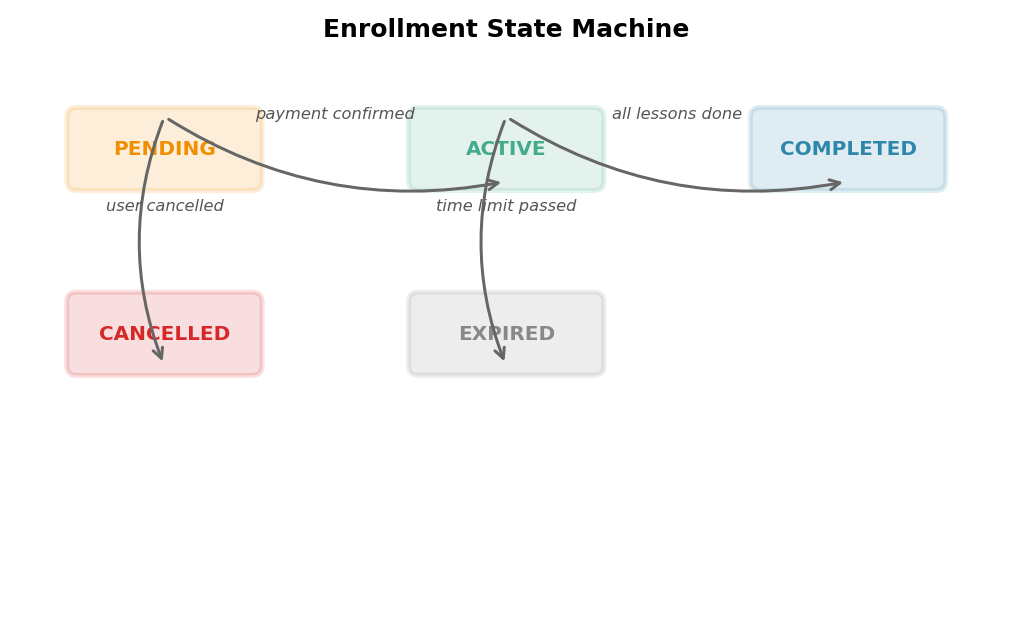
\includegraphics[width=0.6\textwidth]{images/statemachines/enrollment_statemachine.png}
  \caption{Enrollment State Machine}
  \label{fig:enrollment-statemachine}
\end{figure}

Enrollments transition from PENDING to ACTIVE (payment confirmed or free enrollment), from ACTIVE to COMPLETED (all curriculum requirements satisfied), from PENDING to CANCELLED (learner abandoned checkout or manually cancelled), and from ACTIVE to EXPIRED (course access duration limit exceeded, if configured).
